\begin{figure}[h]
\centering
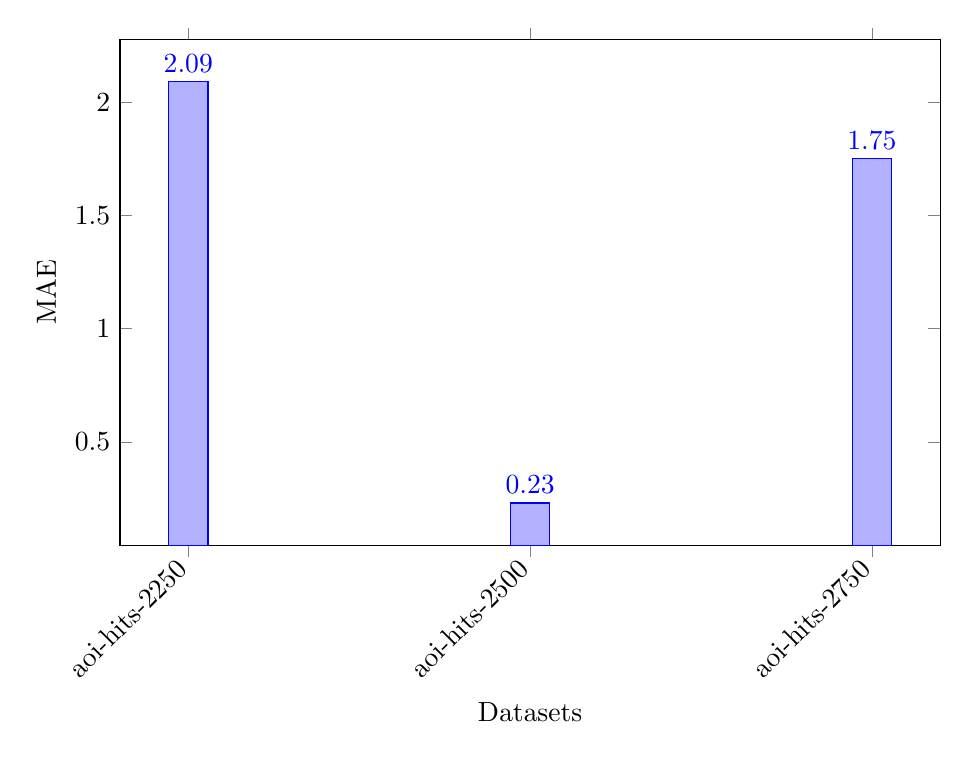
\begin{tikzpicture}
\begin{axis}[
    ybar,
    xlabel={Datasets},
    ylabel={MAE},
    symbolic x coords={aoi-hits-2250, aoi-hits-2500, aoi-hits-2750},
    xtick=data,
    x tick label style={rotate=45, anchor=east},
    width=12cm,
    height=8cm,
    bar width=0.5cm,
    nodes near coords,
]
\addplot coordinates {
(aoi-hits-2250, 2.09)
(aoi-hits-2500, 0.23)
(aoi-hits-2750, 1.75)
};
\end{axis}
\end{tikzpicture}
\caption{MAE por conjunto de datos utilizando parámetros óptimos}
\end{figure}